\documentclass[sigconf]{acmart}
% use \code{foobar} for monospace (instead of \texttt{qux})
\newcommand{\code}{\texttt}

\usepackage{booktabs} % For formal tables
\usepackage{graphicx}
\usepackage[english]{babel}



\begin{document}
\settopmatter{printacmref=false} % Removes citation information below abstract
\renewcommand\footnotetextcopyrightpermission[1]{} % removes footnote with conference information in first column
\pagestyle{plain} % removes running headers

\title{Cryptocurrency Market Prediction Using Twitter}
\subtitle{Final Report}

\author{Will Badart}
\affiliation{%
  \institution{University of Notre Dame}
  \city{South Bend}
  \state{Indiana}
}
\email{wbadart@nd.edu}

\author{Matthew Fabian}
\affiliation{%
  \institution{University of Notre Dame}
  \city{South Bend}
  \state{Indiana}
}
\email{mfabian1@nd.edu}

\author{Shane Ryan}
\affiliation{%
  \institution{University of Notre Dame}
  \city{South Bend}
  \state{Indiana}
}
\email{sryan8@nd.edu}

\author{Mara Staines}
\affiliation{%
  \institution{University of Notre Dame}
  \city{South Bend}
  \state{Indiana}
}
\email{mstaines@nd.edu}


\begin{abstract}
Cryptocurrency as a commodity has proven to be quite volatile, making prediction of market trends highly valuable. In the past year, Our team will leverage the constant stream of tweets discussing cryptocurrency on Twitter in order to build a model that can predict changes in a cryptocurrency's value.
\end{abstract}

\maketitle


\section{Introduction}
Every day, Twitter users produce more than 500 million tweets\cite{sayce}. This makes Twitter an ideal resource for social sensing --- the use of humans as sensors. Users tweet and retweet about events, places, emotions, and more; the aggregation of this data has proven powerful for event detection and prediction. One of the fastest-growing conversations taking place on the platform is over cryptocurrency.

The first decentralized cryptocurrency, Bitcoin, was created in 2009. Currently, over 3500 different cryptocurrencies exist, many simple derivations of Bitcoin. The overall market capitalization of cryptocurrencies has ballooned over the past year to 278 billion dollars. As an example of this rapid growth (and volatility), Bitcoin was being exchanged for \$1,200 per coin in April 2017. It reached a high of \$19,500 per coin in December 2017, and is at \$9,600 per coin as of May 2018.

Because cryptocurrency as a whole is a growing market that is both widely discussed and highly volatile, our team believes that tweets may reflect trends in cryptocurrency value. This belief is rooted in three factors. First, many cryptocurrency investors are speculative. They purchase a cryptocurrency not for its intrinsic value, but because they believe the price will increase and they can later sell it for a profit. Second, these speculative investments are based on news stories, suggestions, and trends in the market. Speculative investors don't purchase cryptocurrencies randomly, rather, they choose to do so because of some sort of input. Finally, we believe that these news stories, suggestions, and market trends can be identified on Twitter before most potential investors have the opportunity to find, analyze, and act on them. In that way, successfully using Twitter data to predict changes in cryptocurrency markets would provide a significant advantage in cryptocurrency trading. 

In this project, we will build a model to predict changes in the value of several major cryptocurrencies based on real-time data from Twitter.


\section{Approach}

\subsection{Data Sources}
Data for this project is collected from Twitter. We streamed tweets using the Twitter API, which allows for tweets to be collected in near real-time. The filtering capability of the Twitter API allowed us to only collect tweets that contain certain keywords. We selected both general keywords (e.g. \code{cryptocurrency}, \code{altcoin}) and keywords for the specific cryptocurrencies being explored (e.g. \code{bitcoin}, \code{BTC}, \code{ethereum}). If a tweet contains one or more of these keywords, our program stored the tweet body as well as important metadata (user ID, timestamp, retweets, favorites, etc.) in JSON format and appended it to a data file.

Many sites provide historical data on cryptocurrency value. We utilized the API of \href{https://www.cryptocompare.com}{CryptoCompare.com} to retrieve cryptocurrency values for the time-span covered by the collected tweets. Initial analysis was completed using only Bitcoin values, but later expanded to include \code{Bitcoin}, \code{Ethereum}, \code{Bitcoin Cash}, \code{Litecoin}, and \code{Rippler}.

\subsection{Methodology}

\begin{figure}[H]
\caption{Flow of data processing}
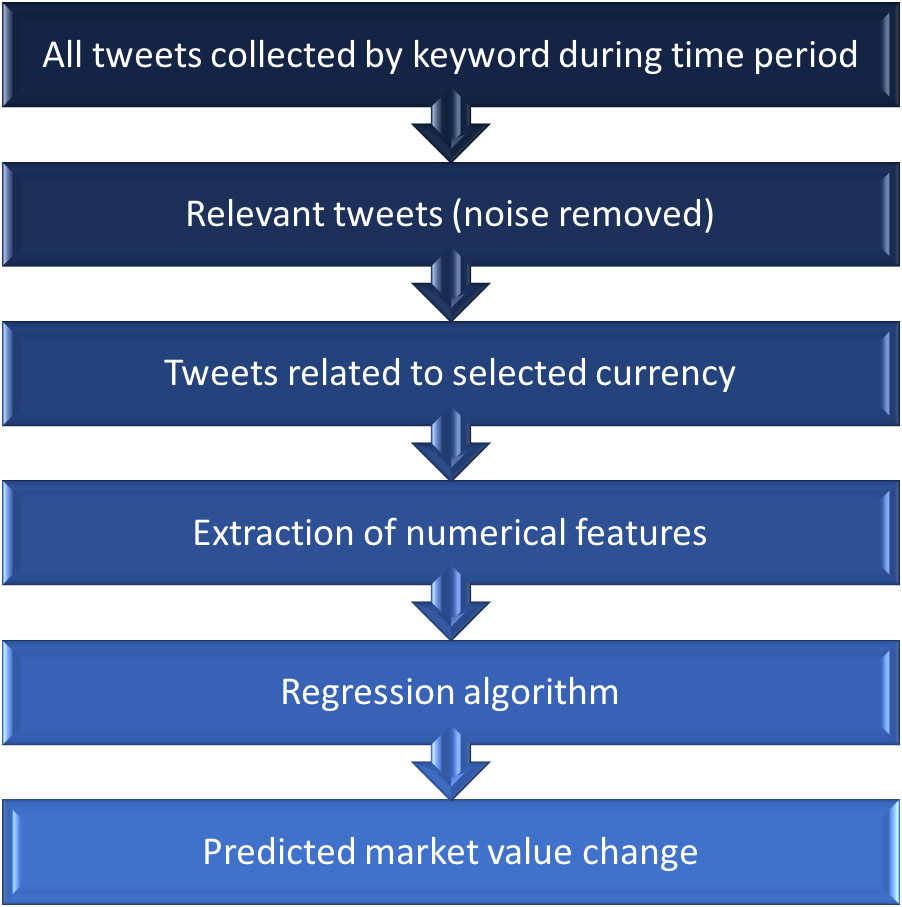
\includegraphics[width=7cm]{chart.png}
\end{figure}

Once data is collected from Twitter, it is cleaned, categorized, and used in a regression model to make currency value predictions (Figure 1). Twitter data is noisy, so the first component of data processing eliminates tweets irrelevant to cryptocurrency which made it past the API filter. Our strategy for this task is to use a clustering algorithm to group tweets as relevant or noise. The data is tokenized using the NLTK TweetTokenizer, which splits the tweet text into distinct words. This submodule is superior to simply splitting the data on whitespace, because it has been coded for the type of text encountered on Twitter. For example, it can split text to preserve common emoticons. The tokenized tweets are used to generate a matrix of token counts. The similarity of two tweets' token count vectors is the measurement used as distance in the clustering algorithm. Tweets are clustered using the KMeans algorithm. This algorithm fits the purpose well, as the number of clusters is known (n=2), and outliers are unlikely due to the character limit imposed on tweets (280 characters). Our research has found that running KMeans on the data in multiple iterations progressively removes more noise from the collected data, with the optimal number of iterations being 3. Figure 2 shows a visual representation of the collected tweets after the third iteration of clustering.

\begin{figure}[H]
\caption{Third Iteration of Relevant/Irrelevant Clustering}
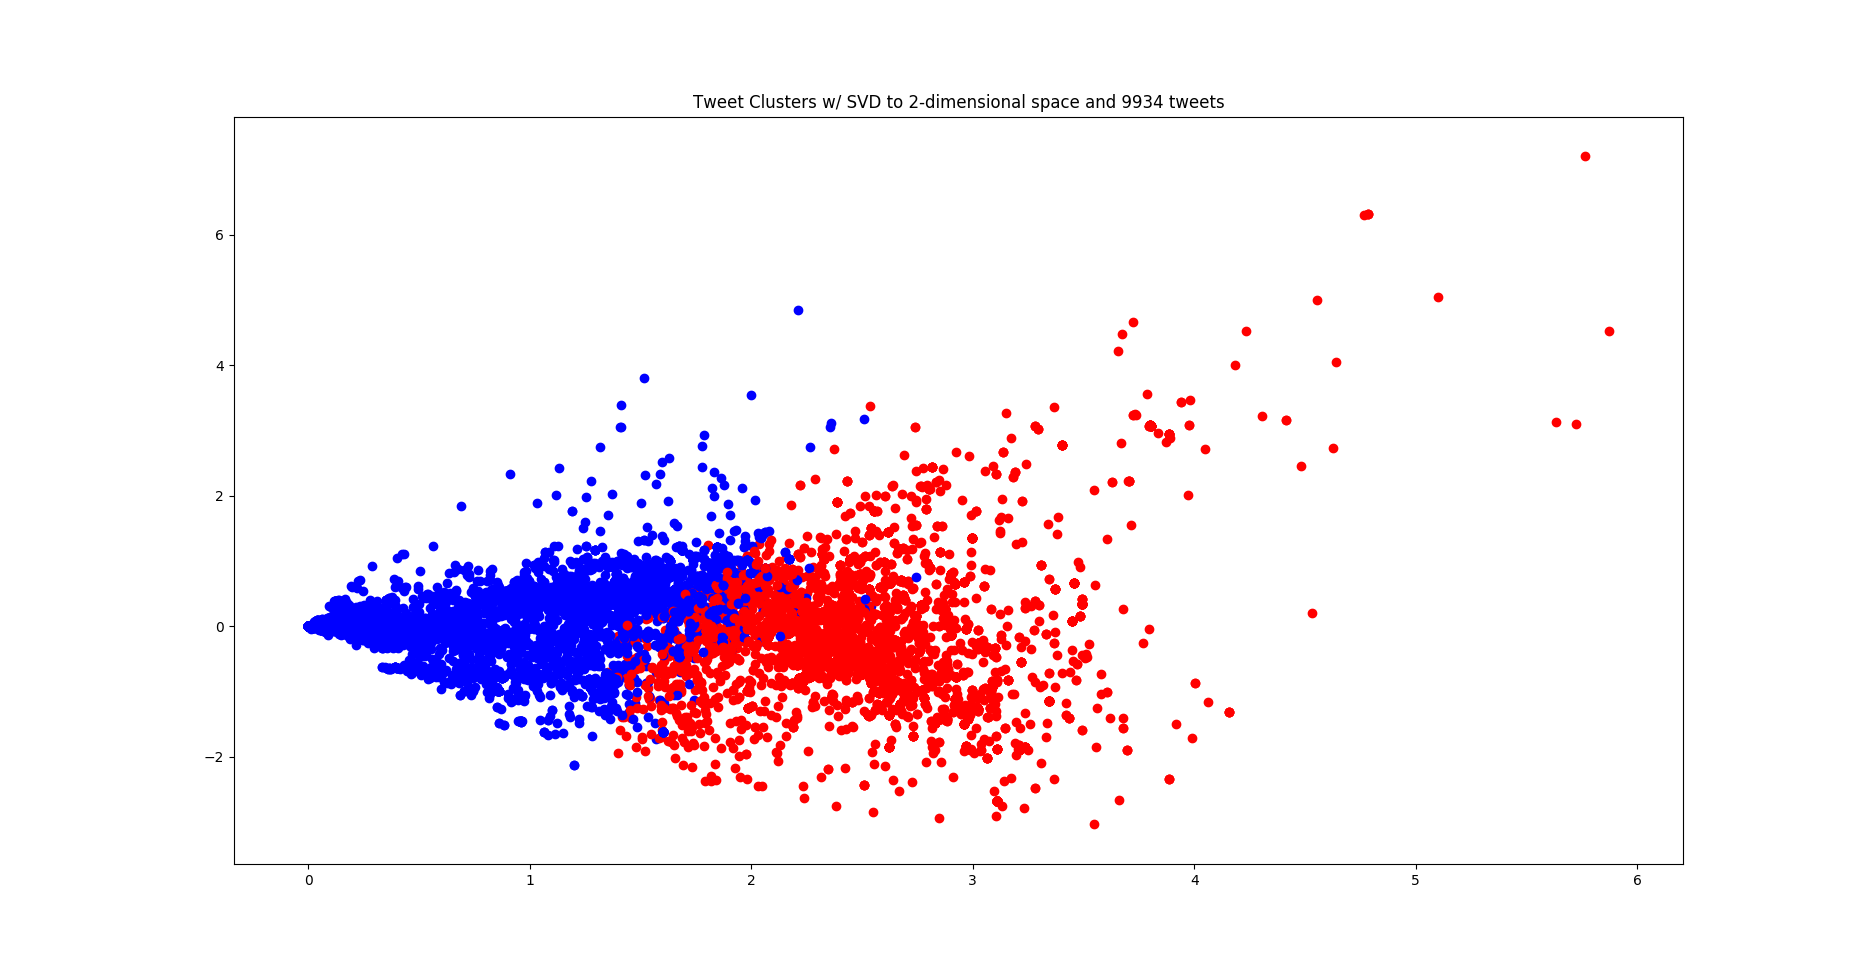
\includegraphics[width=9cm]{3pass.png}
\end{figure}

Once noise was removed and each tweet was labeled with the currency (or currencies) to which it refers, data from the tweets was used to calculate several features for use in the regression model. Features that were calculated for each time-span include the number of tweets, average sentiment of tweets, and standard deviation of tweet sentiment. A tweet's sentiment was calculated using TextBlob, which relies on NLTK. The sentiment is a score from -1 to 1 (where -1 is extremely negative and 1 is extremely positive). A completely neutral tweet would have a sentiment score of 0. Standard deviation of sentiment aims to capture volatility in tweet content. Many neutral tweets would have a standard deviation close to 0, as would equal numbers of highly positive and highly negative tweets. However, the standard deviation for neutral tweets would be significantly smaller than that for tweets with opposing sentiment. 

Due to constraints on time granularity when collecting historical currency prices, tweets are grouped by the hour to generate an instance and calculate its features. Several days worth of data has been collected, allowing us to test the limits of our model in predicting micro-trends. This is especially useful for cryptocurrencies (as opposed to the stock market) due to the excessive volatility that can be found in a coin's price.

For the regression model, we used a Ridge Regression. Initial tests using 24 1-hour data points (1 day) are displayed below in Figure 3. This initial model showed little predictive ability (R-Squared = 0.04).

\begin{figure}[H]
\caption{Regression model given 24 data points for April 6}
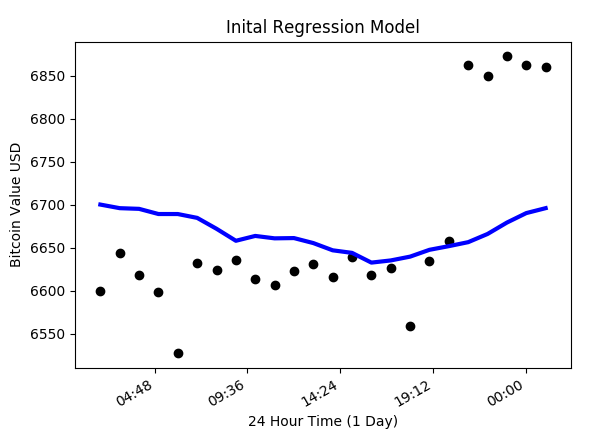
\includegraphics[width=7cm]{regression.png}
\end{figure}

\section{Results}
Evaluation for our model relies on knowing the actual cryptocurrency values over time. Comparison of our predicted changes to actual changes was measured by examining $R^2$. Our goal was to maximize the accuracy of our predictions and minimize the time needed to make a prediction. We found that an hour's worth of tweets provides very little predictive ability. However, for the scope of this course, a successful project will consist of a final model that can take an input period no longer than one day and output an accurate prediction of change in value for a currency.

The accuracy for our model's predictive ability can be measured in two ways: on historical data (on days for which we've collected tweets) and on current data (predicting towards the future). The first method involves building a model on historical data, then predicting the target value for the time-span immediately following the last data point. This prediction was compared to the actual value from CryptoCompare.com. The second method, using current data, streams live data into the model, predicts the target value at the end of the data, then compares the predicted value to the true value once the time of the prediction is reached. The absolute difference between the model's output and CryptoCompare.com's report, $|value_c - value_m|$, can be interpreted as the model's performance.

\section{Discussion}

This research has presented several unique challenges. While Twitter data is plentiful, ensuring quality is difficult. First, technical resources must be chosen carefully to handle the extended, continuous up-time of a Twitter streaming program as well as the large files resulting from this stream. Because the data is temporal, missing a continuous chunk of data can hinder the model. In addition, it is difficult to extract quality text from Tweets. When we conceptualize Twitter, we think of our friends, family, and journalists sharing complete thoughts. In reality, a large number of tweets that are picked up by keyword filters are bots, scams, giveaways, or simply incoherent. With our desire to leverage tweet sentiment, removing this noise becomes extremely important. While we have made significant progress in removing irrelevant tweets, it is a difficult process. What makes a tweet irrelevant is not clear cut, and we do not have any access to ground truths. This project has been a great experience because in the real world, data is messy, noisy, and incomplete. Developing strategies to still find value in this data has helped us all grow immensely over the course of the semester.

\bibliographystyle{ACM-Reference-Format}
\bibliography{milestone}

\end{document}